\section{Massively Learning Activities I - Initial Deployment} \label{section: MLA}
TASI has been contracted by CNMI to create an infrastructure that allows for data analytics on Protected Health Information (PHI). This infrastructure will initially be hosted on-premises, with plans to move towards a hybrid solution in the future. To achieve this, we will be providing a Platform as a Service (PaaS) solution, by hosting SAS Viya 3.5 services on our own hardware and allowing tenants to access and utilize the platform for their own analytics applications.

The tenants, including APCD, CMNI, CMA, Criminal Justice, and several Education environments, will provide the necessary data, which will be submitted to an ETL data pipeline for processing before being sent to SAS on-prem servers. Once the data has been processed, tenants may perform data analytics using advanced algorithms in SAS programming language.

To ensure secure operations, we will configure the security relationships between the software, hardware, and tenants using LDAP, security groups, encryption  and other related tools. Our goal is to architect a high-performance infrastructure that allows for advanced data analytics while maintaining the confidentiality and security of PHI.

Due to SAS being a time sensitive project, the initial deployment will have SAS suites and VMs installed on existing hardware, with plans to migrate the infrastructure to newly acquired hardware in the future.

The initial deployment of SAS technologies will expect 4 tenants:
\begin{enumerate}
    \item Commonwealth of the Northern Mariana Islands (CNMI)
    \item All-Payer Claims Database (APCD)
    \item Centers for Medicare \& Medicaid Services (CMA)
    \item Med-Quest
\end{enumerate}

\subsection{Planning}

The System Development Life-cycle (SDLC) is a project management model that defines different stages that are necessary to bring a project from conception to deployment and later maintenance. The SDLC model consists of several phases, which typically include requirements gathering, design, development, testing, deployment, and maintenance. The specific activities within each phase may vary depending on the project and the organization, but the basic principles are the same. The SDLC model is a flexible framework that can be adapted to suit the needs of different projects and organizations. It provides a systematic approach to software development that helps ensure that software is built efficiently, effectively, and with minimal risk.

Massively Learning Activities will follow a similar variation to the SDLC project management model where each SDLC stage will correspond to a subsection in this chapter. 

\subsection{Pre-Deployment Workstream I}

The Pre-Deployment Workstream is divided into two phases: Requirements of Analysis and Deployment Design. 

In phase 1, ongoing project management tasks will be performed, including preparing a project plan and assigning appropriate resources. SAS will send billable work hours log for UHTASI to verify based on project plan. Additionally, SAS will send Pre-Install Requirements Document to UHTASI for completion. Both parities will ensure environmental readiness for install by reviewing the completed Pre-Install Requirements Document. 

In phase 2, the design for the installation of SAS software suites will be completed. The design will cover the configuration of VMs for SAS Viya 3.5, SAS 9.4, and relevant connections to storage pools. 

\subsubsection{Requirements of Analysis}
Refer to ECC Sizing Document. (Pre-Install Checklist)

\subsubsection{Deployment Design}

For the initial deployment of MLA, we will be installing SAS Viya 3.5 3.4, SAS 9.4, and SAS DMA on TASI's existing infrastructure\footnote{Infrastructure is used to describe existing hardware available to use on-premises at TASI/PHIDC.}. Specifically, we will use the Dell PowerEdge FX2 Enclosure, which is already available in TASI's NOC to install SAS software. This 2U hybrid rack-based computing platform combines multiple blades\footnote{Blades are complete servers in a smaller form factor that have their own CPU(s), memory, storage, and networking components.} into a single enclosure, making it an efficient and cost-effective solution for our needs.

The PowerEdge FX2 Enclosure is connected to a storage pool with XXTB capacity that is holding a copy of ePHI data. Each blade in the enclosure runs ESXi 6.7 as the host operating system and is equipped with 12 CPU(s) and XX cores, 256GB of RAM, and XXGB of personal storage. We will logically separate these resources to create a multi-tenant environment, with virtual machines (VMs) managed through vCenter (and later through SAS). The VMs responsible for a CAS role will use RHEL 7.X as the host operating system. 

Initially, four tenants will be deployed: CNMI, APCD, CMA, and Med-Quest. Each tenant will have their own deployment configuration based on their respective requirements. CNMI and APCD will be configured in a 5-server\footnote{5 Server: (1) Primary CAS Controller, (2) Backup CAS Controller, (3) CAS Worker 1, (4) CAS Worker 2, (5) CAS Worker 3} environment, while every other tenant will be configured in a 3-server\footnote{3 Server: (1) Primary CAS Controller, (2) Backup CAS Controller, (3) CAS Worker 1} environment. Additional tenants will be added during the migration stage of MLA.

\begin{figure}[H]
    \centering
    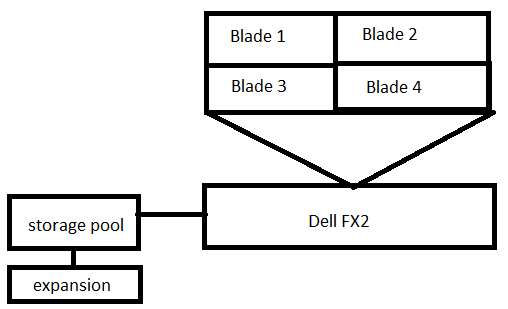
\includegraphics[scale = 0.75]{images/currentENV.png}
    \caption{TASI On-Premise Environment \textcolor{red}{(needs VISIO)} }
    \label{Current ENV}
\end{figure}

The configuration of SAS technologies is affected by the need for high availability and redundancy, optimization, and adherence to security and compliance requirements.

\begin{enumerate}
    \item High Availability and Redundancy
    \begin{itemize}
        \item Consider that although virtualizing the CAS Controller and Backup Controller on the same hardware can offer several benefits, such as cost savings, simplified management, and easier backup and recovery processes, it will be better to virtualize them on separate hardware to provide high availability and redundancy of CAS controllers (Figure 6.2), in the case of unexpected downtime. As for CAS Workers, it is recommended to virtualize them on separate hardware to reduce resource conflicts but it is not necessary. 
    \end{itemize}
    \item Optimization
    \begin{itemize}
        \item The performance overhead of using SAS Viya 3.5 and CAS on VMs instead of dedicated hardware can depend on several factors including workload characteristics, available hardware resources, and the virtualization technology used.
        \textcolor{red}{In section 6.3.1, if the advantage of distributing the SAS components across blades is for load balancing, it would be good to include a comment to that effect -- otherwise, it would probably be more efficient to have them all on the same blade.}
    \end{itemize}
    \item Security and Compliance
    \begin{itemize}
        \item In a logically separated multi-tenant environment, MLA must ensure network and data isolation between each tenant, data encryption for data at rest and in transit, a well configured access control list for hardware and software, and compliance certification for handling PHI data (i.e., HIPAA, PCI DSS, SOC 2, HITECH, Hawaii Information Privacy Act, etc). 

    \end{itemize}
\end{enumerate}
\begin{figure}[H]
    \centering
    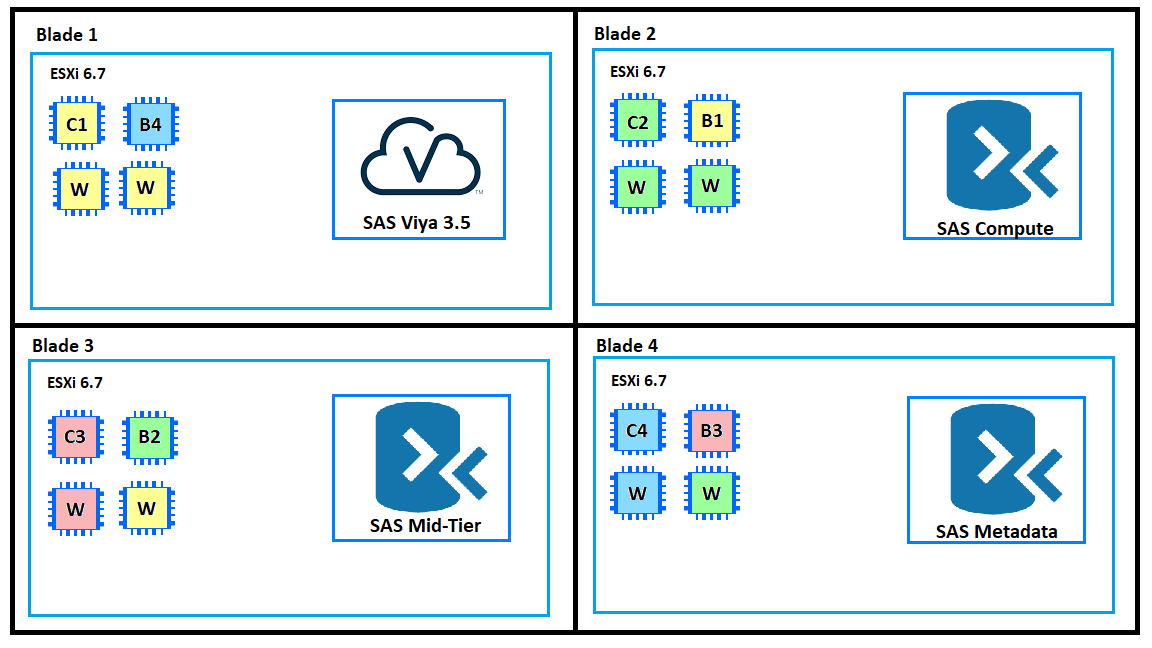
\includegraphics[scale = 0.52]{images/initial-deployment-diagram.png}
    \caption{Initial Multi-Tenant Deployment \textcolor{red}{(needs VISIO)} }
    \label{Initial Multi-Tenant Deployment}
\end{figure} 

To maximize resource efficiency, CAS nodes will be evenly distributed across each blade, where a blade will consist of one controller, one backup controller, and two workers. The controller and backup controller, configured on the same system, will belong to separate tenants. The workers will also belong to separate tenants but each blade will have at least one related controller and worker per system. 

Subsequently, four additional VMs will be created to support the installation of SAS Viya 3.5 and SAS DMA. SAS Viya 3.5 will be installed as software on top of a RHEL 3.7X VM instance, in Blade 1. SAS DMA consists of three software components that will installed as software on top of Windows Server 2019 VM instances, in Blades' 2, 3, and 4. 

\subsection{Deployment and Prototyping I (Initial)}

April 18, 2023:
SAS 9.4 is installed first on TASI system. It is configured this way on blade 1. 

\subsection{Testing \& Integration I}

\subsection{Operations and Maintenance I}